\documentclass[12pt]{report}
\usepackage[utf8]{inputenc}
\usepackage[french]{babel}
\usepackage[T1]{fontenc}
\usepackage{amsmath}
\usepackage{amsfonts}
\usepackage{amssymb}
\usepackage{graphicx}
\usepackage{titlesec}
\usepackage{caption}
\usepackage{titling}
\usepackage{booktabs}
\usepackage{enumitem}
\usepackage{eurosym}
\usepackage{epigraph}
\usepackage{hyperref}
\usepackage{fontspec}
\usepackage{ragged2e}
\usepackage{parskip}
\usepackage{wrapfig}
\usepackage{calc}
\usepackage{float}

\graphicspath{ {../img/} }
\setlength{\droptitle}{-10em}
\titleformat{\chapter}[hang]{\normalfont\huge\bfseries}{\thechapter. }{0em}{}

\begin{document}

\title{
	{\vspace{3em}\protect\centering\protect
\includegraphics[width=0.9\textwidth]{pacification_vector.pdf}}\\
	{\vspace{4em}\Huge Rapport de soutenance}\\
	{\large Brainless Devs}
}
\author{
	Thibault Allançon\\
	Valérian Fayt
	\and
	Antoine Gonzalez\\
	Cédric Parpet}
\date{
	{\vfill\protect\centering\protect
\includegraphics{logo_short_vector.pdf}}\\
	Dossier Projet Informatique\\
	Info-Sup EPITA\\
	Mars 2018
}

\maketitle
\tableofcontents

\chapter{Introduction}

Cette première phase de développement de \textit{Pacification} aura été assez riche d'expérience. En effet, il a fallu partir de rien et poser les fondations de notre jeu. Cela aura été une phase de découverte de notre environnement de travail, d'expérimentation pour notre partie réseau, de réflexion pour notre partie gameplay, et de préparation pour notre partie graphique. Toutefois, nos objectifs ont étés atteints. La map et le réseau sont pour le moment fonctionnels, nous avont nos premiers assets qui pourront ensuite être réutilisés afin de gagner du temps, et l'organisation du gameplay et des éléments du jeu est claire.

\begin{figure}
    \centering
    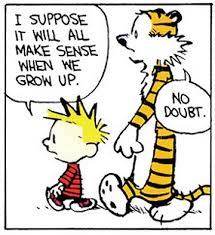
\includegraphics[width=0.6\textwidth]{project_mood_S1}
    \caption*{\textit{Calvin and Hobbes}, Bill Watterson}
\end{figure}

\chapter{Cahier des charges}

Le cahier des charges nous semble toujours satisfaisant, nos objectifs sont atteignables, et il n'y a selon nous rien à ajouter au jeu qui n'ait pas été mentionné dans le cahier des charges. La répartition des tâches est convenable, bien que certains changements auront lieu pour la seconde période : notamment Antoine et Valérian qui deviendront suppléants UI pour assister Cédric qui sera très occupé par les assets, ainsi qu'établir l'interface anglais/français dans le jeu. Les assets faits à la main, bien que longs à réaliser, sont très satisfaisants et l'investissement en temps en vallait la peine. En ce qui concerne l'IA, les 30\% prévus étaient ambitieux sachant qu'il n'y a pas encore suffisamment d'éléments de gameplay implémenté.

\chapter{Avancement}

\section{Map (Thibault)}

L’ensemble du jeu repose entièrement sur la carte, il était donc fondamental de s’y attaquer le plus tôt possible et d’implémenter rapidement le strict nécessaire pour développer le reste du jeu.

La particularité de la map étant qu’elle est constituée d’hexagone, il fallait donc correctement prendre cela en compte tant pour l’aspect graphique (rendu visuel, pavage) que l’aspect technique (nouveau système de coordonnées/déplacement, gérer correctement les relations de voisins).

\begin{figure}[H]
    \centering
    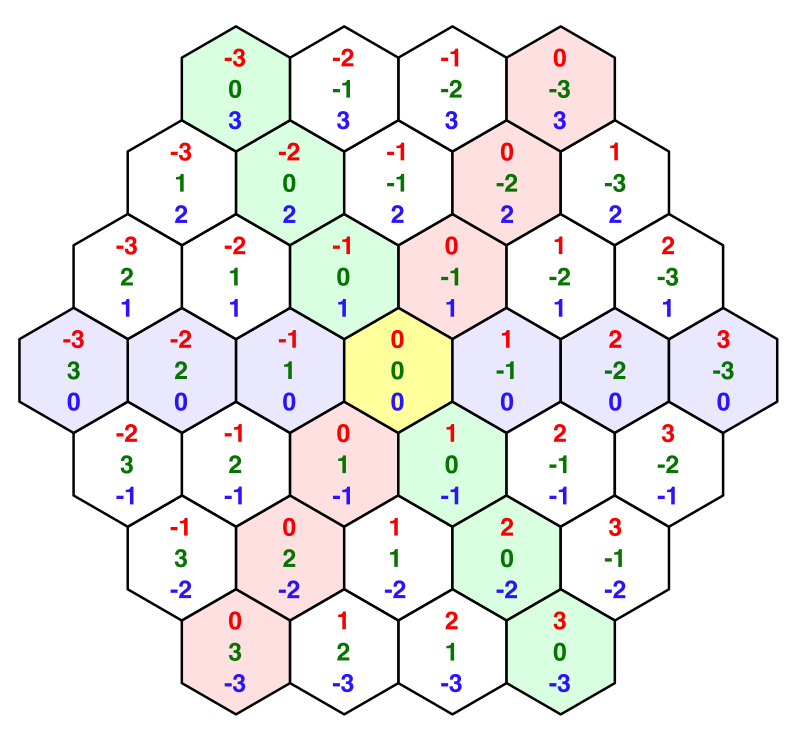
\includegraphics[width=0.5\textwidth]{cubic_coordinates}
    \caption{Système de coordonées et axes}
\end{figure}

De plus la carte est découpée en chunks afin de faciliter le rendu et avoir une meilleur fluidité sur des tailles de carte conséquente. En effet, utiliser un seul mesh pour toute une carte n’est clairement pas envisageable, surtout en anticipant le multijoueur, il faut donc découper cette dernière en chunks qui ont chacun leurs propres mesh. Lors d’une mise à jour de la map, il suffit alors de mettre à jour quelques chunks et non toute la carte (ce qui allège considérablement le rendu graphique).

Actuellement la carte présente différentes caractéristiques modifiables : des biomes pour les cases, possibilité de créer des montagnes d’une hauteur variable, création de routes pour relier des cases entre elles. Tout ceci a nécessité une manière d’interagir et de se déplacer sur la carte en jeu (flèches directionnelles, détection du clic et identification de la case sélectionnée, zoom).

\begin{figure}[H]
    \centering
    %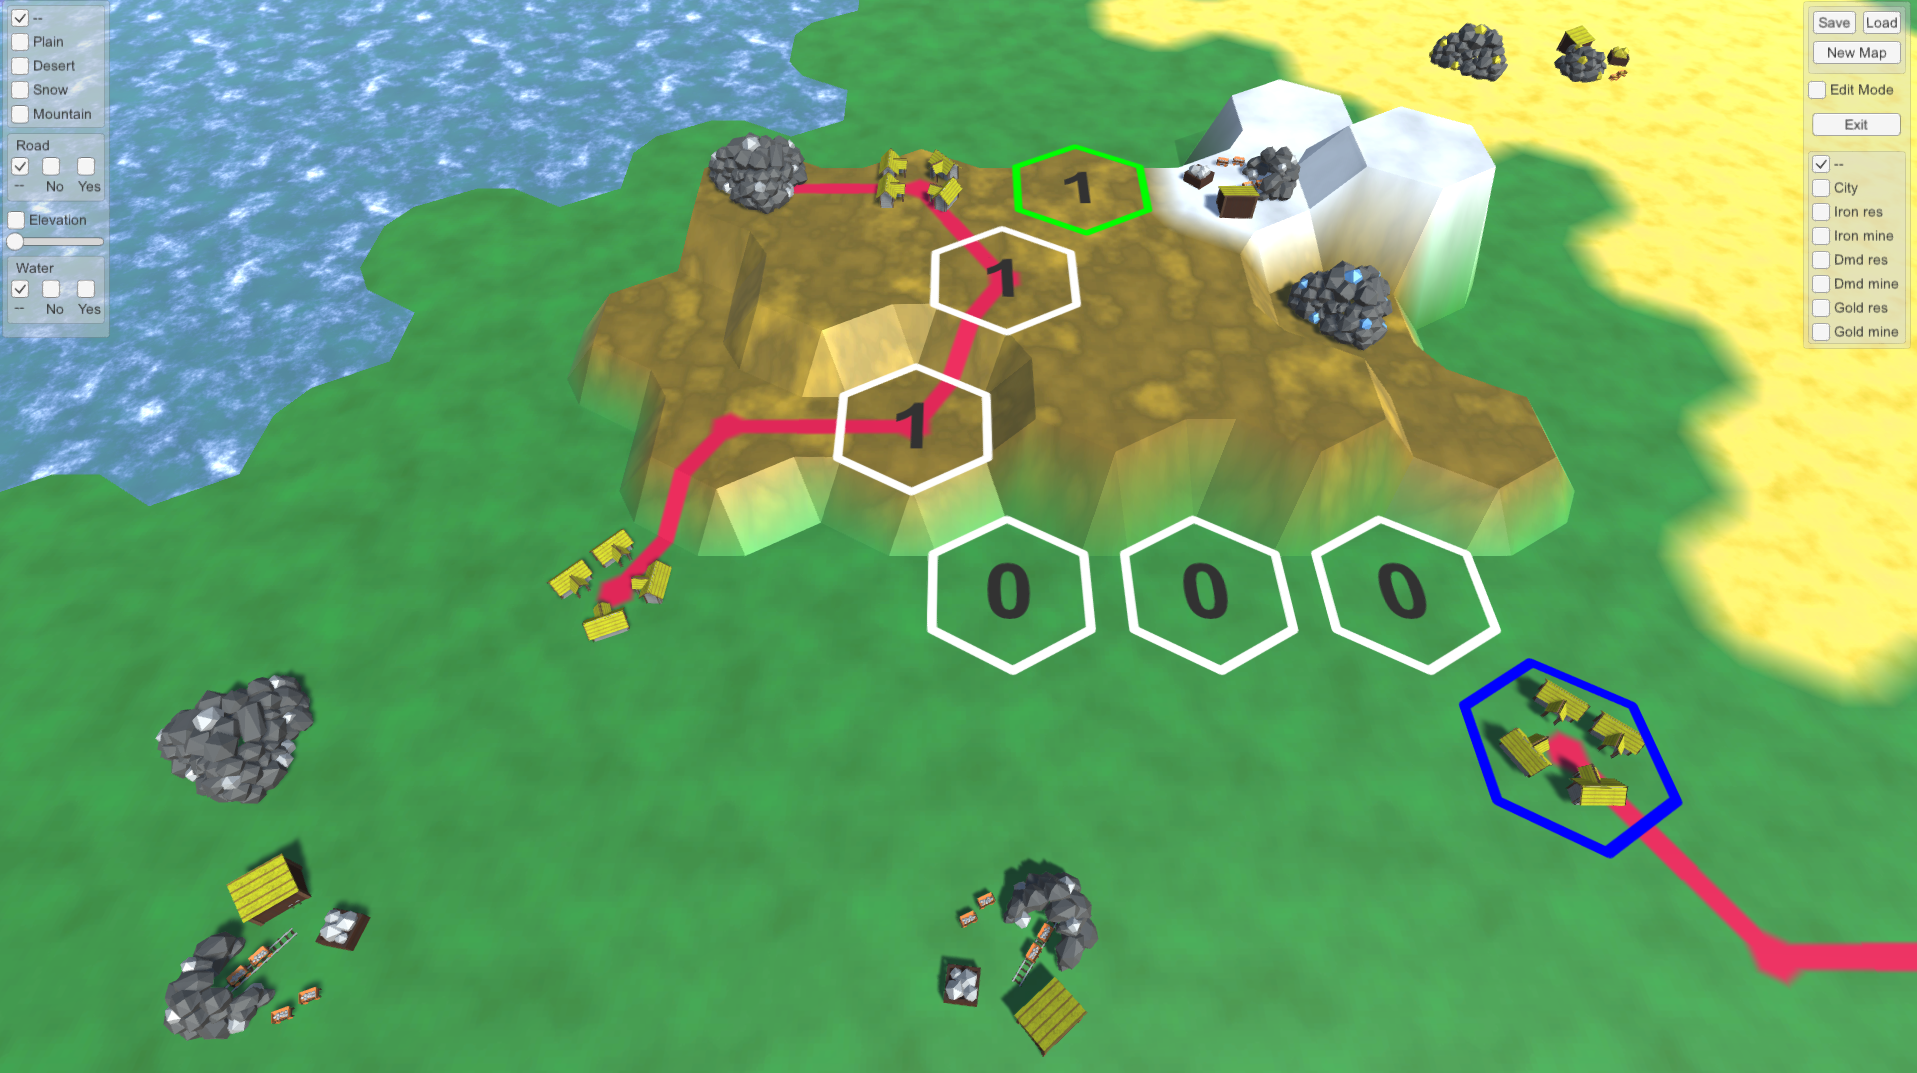
\includegraphics{map_features}
    %\caption{Exemple de map}
\end{figure}

Le système de sauvegarde et de chargement est aussi en place, il pourra permettre d’avoir un mode de création de ses propres cartes qu’on pourra ensuite sélectionner en solo ou en multi pour jouer dessus.

\begin{figure}[H]
    \centering
   %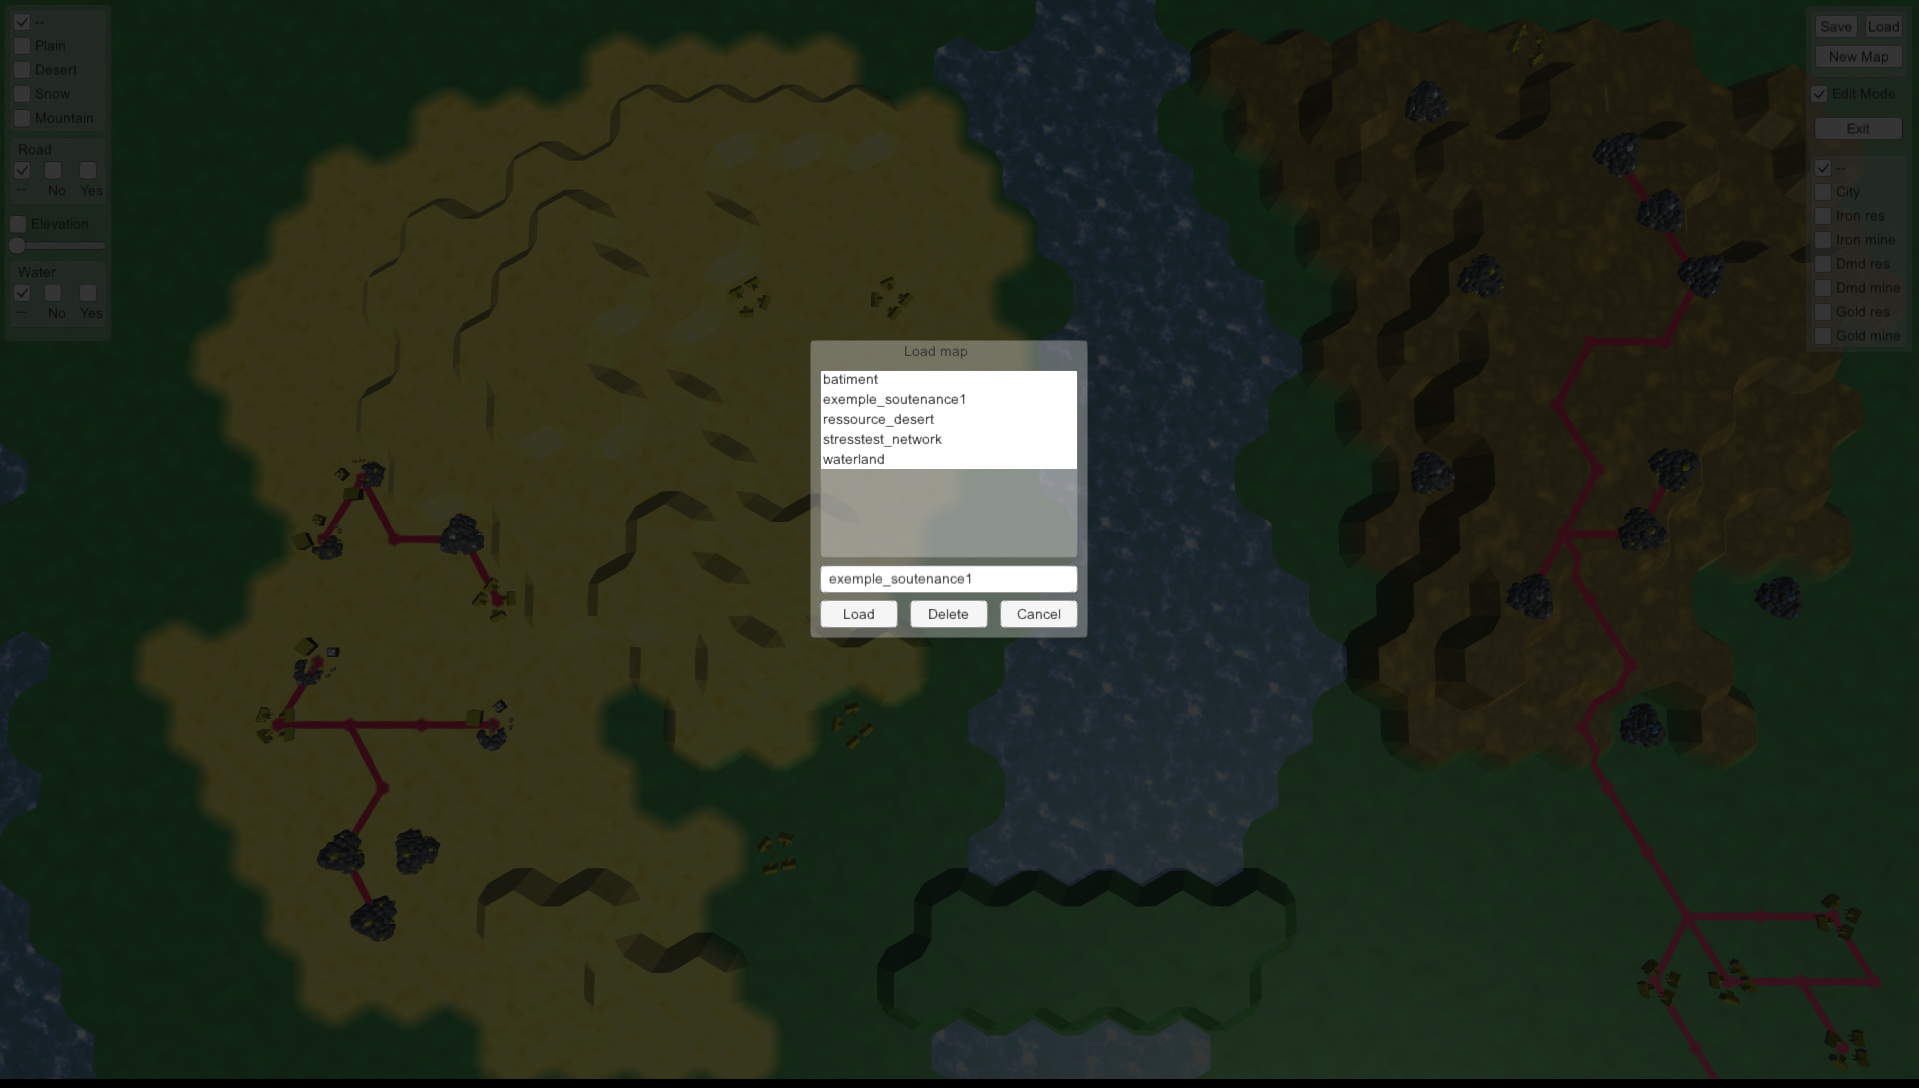
\includegraphics{map_save_load}
    %\caption{Menu de sauvegarde/chargement}
\end{figure}

Un premier pas vers le support complet des unités a été fait en créant le système de pathfinding pour se déplacer sur la carte (prenant en compte des aspects tel que l’élévation, les routes, etc.). Le C\# ne disposant pas d’une classe pour créer des tas, il a fallu commencer par l’implémentation d’une file à priorité afin de mettre en place l’algorithme A\*. Ce dernier est une variante de l’algorithme de Dijkstra pour calculer le plus court chemin dans un graphe pondéré positivement, et se base sur une heuristique afin d’accélérer la recherche de ce chemin.

\begin{figure}[H]
    \centering
    %\includegraphics{pathfinding}
    %\caption{Pathfinding}
\end{figure}

\section{Réseau et multijoueur}

L’implémentation du multijoueur étant essentielle pour le bon déroulement du jeu, il était prioritaire de le rendre fonctionnel. Contrairement à ce qui avait été envisagé, le multijoueur proposé basiquement par Unity ne nous convenait pas, car ne nous permettait pas d’avoir un contrôle total sur cette partie. De plus, la perspective d’apprentissage était bien plus intéressante en passant par un codage par soi-même du multijoueur plutôt que d’utiliser une base déjà préfabriquée. 
Ainsi, le multijoueur pour lequel nous avons opté est constitué d’un serveur et de clients. Le serveur est démarré lorsqu’un joueur héberge la partie. Les clients quant à eux, sont activés automatiquements sur les ordinateurs des joueurs tentant de se connecter à un serveur pour rejoindre une partie. À noter que le joueur qui héberge possède lui aussi un client qui se connecte directement au serveur, au démarrage de celui-ci.

Lorsque le serveur est démarré, il commence à écouter dans l’attente de tentatives de connexions. Tant que le nombre de joueurs souhaité (de 2 à 8) n’est pas atteint, il continue d’attendre des connexion. Les clients se connectent à ce serveur à l’aide de l’adresse IP de l’hôte. A chaque tentative de connection d’un client, le serveur lui demande de s’identifier, en lui envoyant en même temps la liste des identifiants des clients déjà connectés. Une fois l’identifiant obtenu, il est transmis aux autres clients. Si l’un des clients se déconnecte, le serveur transmet cette informations aux clients encore en ligne. Ce processus permet à tous les joueurs de savoir à tout moment qui est connecté sur la partie.

\begin{figure}[H]
    \centering
    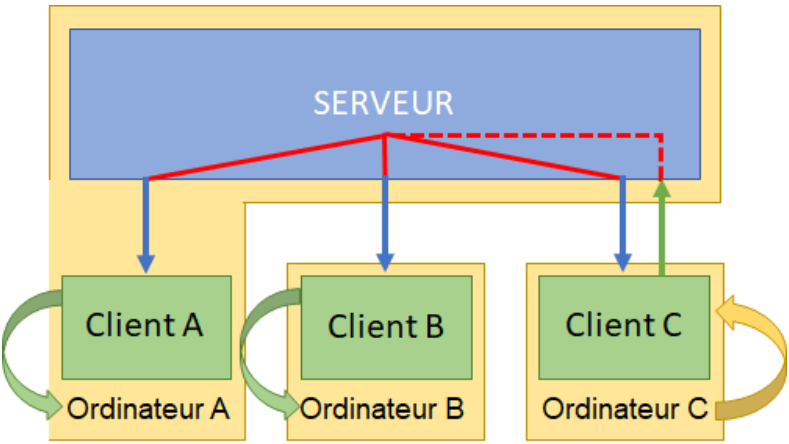
\includegraphics[width=0.8\textwidth]{shema_multi}
    \caption{Shéma fonctionnel du réseau}
\end{figure}

Quand le nombre de joueurs souhaité est atteint, le serveur n'accepte plus de connexion et transmet aux clients un message annonçant le début de la partie, ce qui a pour effet de démarrer celle ci à la réception par les clients.

Pendant le jeu, les échanges sont effectués via un processus de sérialisation. Lorsqu’un joueur effectue une action, celle-ci est sérialisé sous forme de string puis envoyé au serveur qui se charge de dispatcher correctement le-dit message aux autres joueurs. À la réception d’un message, le client va reproduire l’action que ce message décrit. Le type d’action est définie par les quatres premiers caractères du message transmis : Le premier caractère indique le type de l’expéditeur (S pour le serveur, C pour un client) et les 3 suivant indiquent le type d’action.

\begin{center}
	\begin{tabular}{c|c}
		\toprule
		\textbf{Caractères}  & \textbf{Action}\\ 
		\midrule
		WHO & Demande d’identification \\
		IAM & Réponse d'identification \\
		CNN & Nouvelle connection \\
		DEC & Déconnection d’un client \\
		MAP & Transmission de la map \\
		END & Annonce de la fin d’un tour \\
		YGO & Autorisation de début de tour\\
		MOV & Mouvement d’unité effectué\\
		BDC & Construction d’un bâtiment\\
		BDM & Mise à jour d’un bâtiment\\
		EDI & Edition de la map\\
		MSG & Message global\\
		MSP & Message privé\\
		MSE & Erreur de destinataire du message\\
		\bottomrule
	\end{tabular}
\end{center}

\vspace{1em}

Ce système a ainsi permis la mise en place d’un suivi de l’état des clients (connecté / déconnecté) synchronisé sur tous les appareils, ainsi que la base d’un système de chat entre les joueurs (public et privé) mais aussi plus particulièrement la synchronisation des éditions de la map de jeu.

La latence qui pourrait survenir avec ce système n’est pas un problème dans le cas de ce projet, car il ne s’agit pas d’un jeu nécessitant une synchronisation en temps réel etant donné que les parties se déroulent en tour par tour.

Un exemple du processus pouvant être celui-ci :

\begin{itemize}[label=\textbullet]
	\item Le joueur \textit{player\_A} déplace une unité (numéroté 3) de la case $(5;3)$ vers la $(5;5)$
	\item Le client envoie le message\textit{ “CMOV|3\#5.3\#5.5”}
	\item Le serveur reçoit et renvoie aux clients\textit{ “SMOV|player\_A\#3\#5.3\#5.5”}
	\item Les clients reçoivent le message et le décryptent pour déplacer l’unité du \textit{playerF\_A}
\end{itemize}

\section{Gameplay (Antoine)}

Pour le moment, le gameplay était en phase de réflexion. Avant de commencer à implémenter les différents éléments du jeu, il était important pour moi de tout représenter visuellement de manière organisée afin de faire le maximum d’ajustements sans avoir à modifier de code (limitant ainsi les bugs et conflits).

L’élément le plus important est la hiérarchie des classes, qui permet de voir clairement quelle classe hérite de quelle autre classe, afin d’anticiper les héritages et d’éviter les attributs inutiles. Les autres liens entre les classes (contient/produit/énumérations de types) permet d’anticiper des attributs et méthodes, en gardant le réseau et la map en tête pour chaque méthode. Enfin, l’organisation du diagramme permet de rapidement visualiser quelles classes sont à travailler en priorité, et d’identifier l’origine de certains bugs pouvant survenir au cours du développement (selon leur dépendance).

\begin{figure}[H]
    \centering
    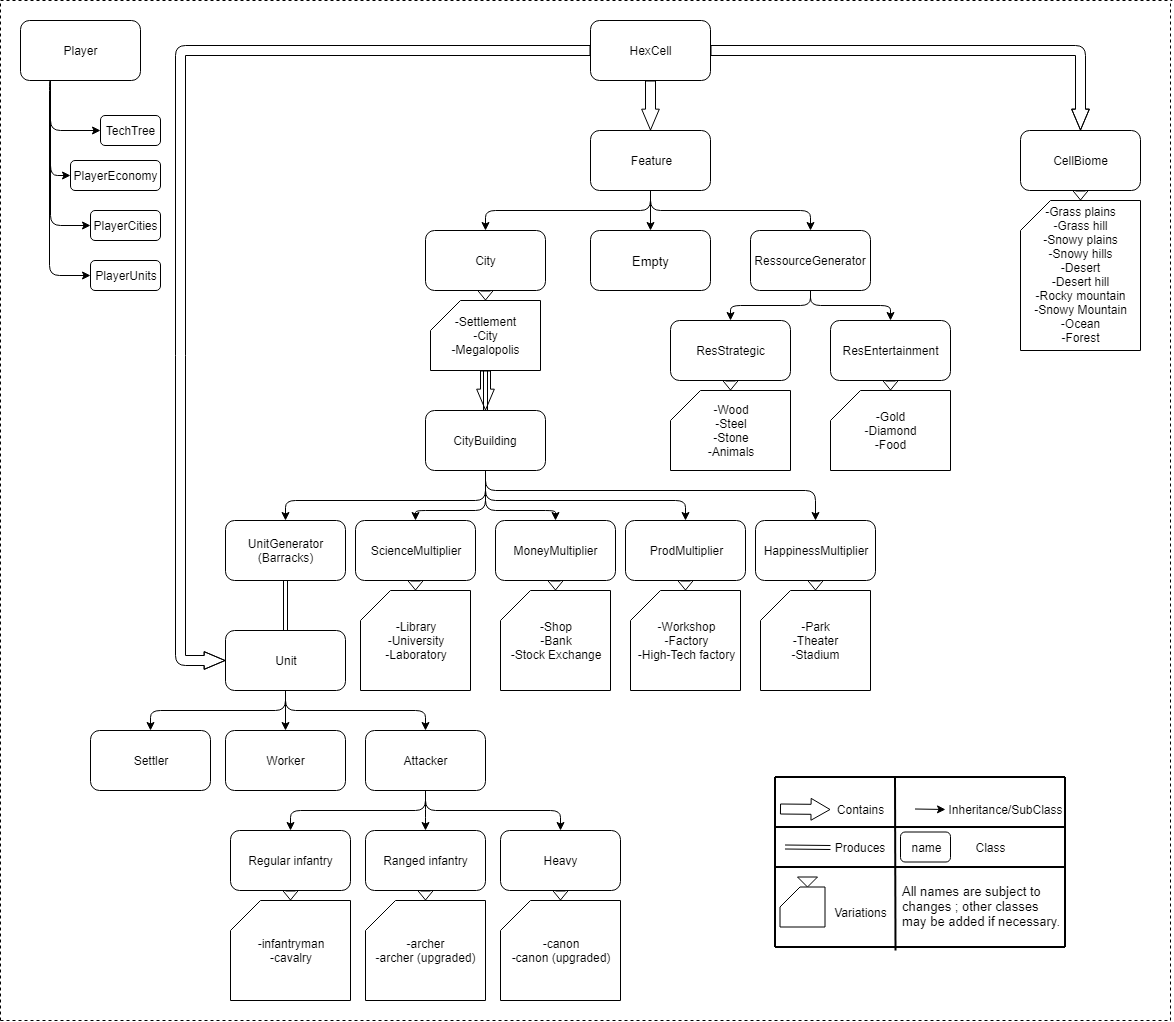
\includegraphics[width=1\textwidth]{DIAG_CLASSES__hierarchy}
    \caption{Hiérarchie des classes}
\end{figure}

Certains éléments ont commencé à être équilibrés (notamment les unités et les biomes), afin d’identifier un maximum d’attributs nécessaires à leur implémentation, et de paramètres à ajuster sur la map. Cet équilibrage semble pour le moment satisfaisant, mais sera probablement modifié pour la dernière soutenance, une fois que le jeu sera terminé et qu’il ne restera plus qu’à faire du \textit{“fine tuning”} suite à des tests en conditions réelles (les paramètres actuels n’étant issus que de calculs et de graphiques).

Nous avons par exemple ces différents tableaux qui donnent une idée précise de comment les unités interagissent entre elles, comment leurs statistiques évolueront au fil de la partie, et comment chaque biome affecte le jeu.

\begin{figure}[H]
    \centering
    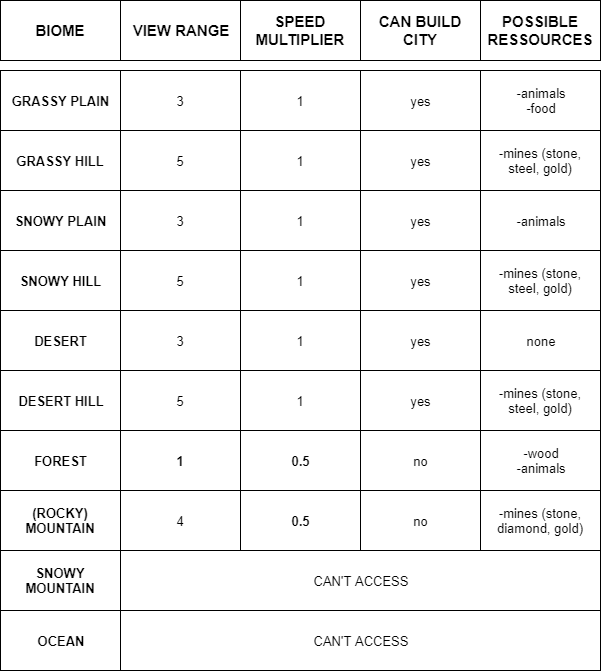
\includegraphics[width=0.9\textwidth]{DIAG_BIOMES__effects}
    \caption{Effets des biomes}
\end{figure}
\begin{figure}[H]
    \centering
    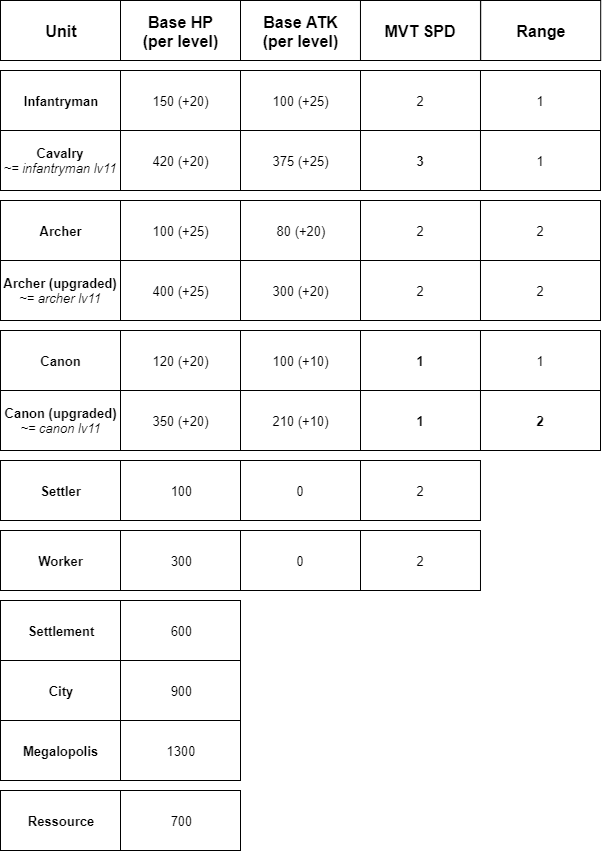
\includegraphics[width=0.9\textwidth]{DIAG_TROOPS__stats}
    \caption{Statistiques par niveau}
\end{figure}
\begin{figure}[H]
    \centering
    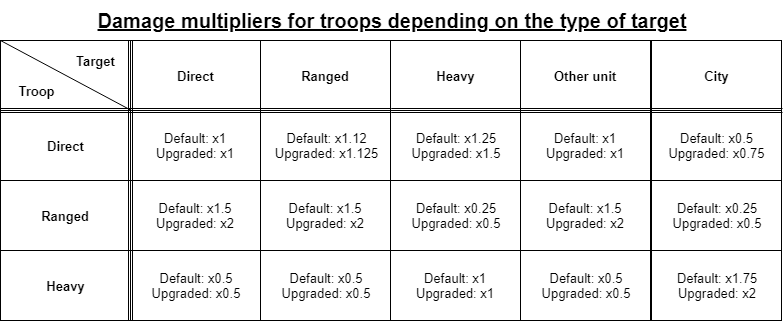
\includegraphics[width=0.9\textwidth]{DIAG_TROOPS__damage_multipliers}
    \caption{Multiplicateurs de dégats en fonction des cibles}
\end{figure}

En somme, le gameplay est presque entièrement préparé, les différentes classes sont prévues et organisées, les attributs et méthodes sont listés, et il y a un début d’équilibrage. Il ne reste maintenant qu’à implémenter cela, ajouter les éléments qui ont pus être oubliés, et équilibrer le tout en testant le jeu.

La partie économie n'a pas été réalisée pour le moment: elle nécessitera des tests en direct et n'est pas  indispensable pour avoir un début de jeu. Je m'occuperais donc de l'équilibrage des ressources, des villes et de l'arbre technologique dans les semaines qui viennent.

\section{Assets (Cédric)}

Pour le design du jeu nous avions pensé à un style un peu “cartoon” constitué de modèles 3D comportant peu de polygones. La principale raison étant que les objets sont ainsi plus facile à produire puisque tout est fait par nous même via le logiciel blender. Le choix de blender était évident de par sa gratuité et parce que l’un des membres du groupe était déjà habitué à ce logiciel. Pour importer les modèles 3D de blender à unity il a fallu les exporter en format FBX ce que blender peut faire facilement.

La ville d’un joueur évoluant au fil du temps suite à ses améliorations technologiques et à l’augmentation de sa population, il faut donc créer plusieurs modèles pour le même objet. Les unités sont elles aussi destinées à évoluer au fil des améliorations technologiques du joueur. Les unités et batiments auront une apparence inspirée de l'antiquité et/ou du moyen-âge. chaque type d'unité offensive aura deux apparence, et les villes en auront trois, à chaque fois selon leur niveau/état (voir tableaux dans la partie Gameplay).

La modélisation est chronophage, mais une fois les premiers modèles créés, les suivants peuvent les réutiliser et ainsi leur création est de plus en plus rapide.

Concernant les unités humaines, celles-ci se basent sur un modèle créé par nous même et auront la même armature de base.

\begin{figure}[H]
    \centering
    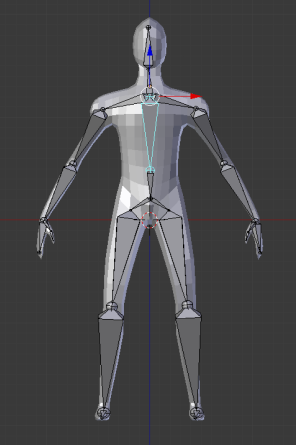
\includegraphics[width=0.3\textwidth]{RefUnitWthArmature}
    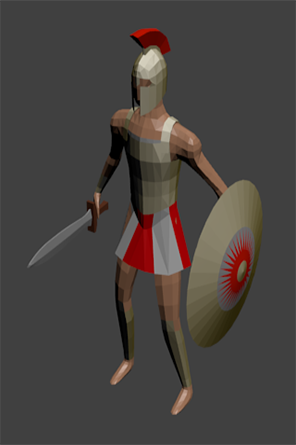
\includegraphics[width=0.3\textwidth]{Swordmen}
    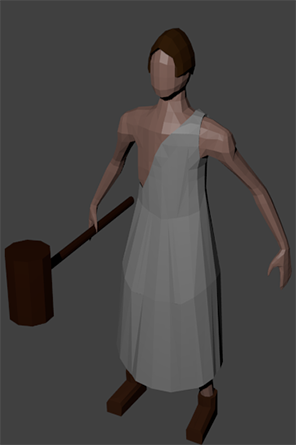
\includegraphics[width=0.3\textwidth]{Worker}
    \caption{Unités et armature}
\end{figure}

La priorité a été mise sur les ressources de la carte et la ville, ainsi que sur les textures de la carte correspondant aux différents biomes. Celles-ci ont été faites grâce à un plugin de Unity “NumberFlow” qui permet de générer des textures de manière procédurale.

\begin{figure}[H]
    \centering
    
\includegraphics[width=0.2\textwidth]{Plain_Tex}
    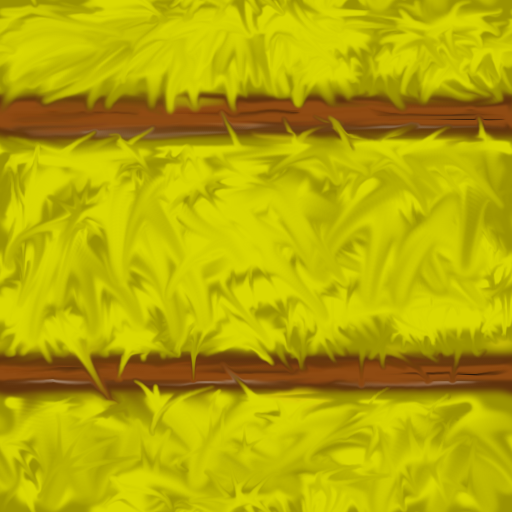
\includegraphics[width=0.2\textwidth]{StrawRoof}
    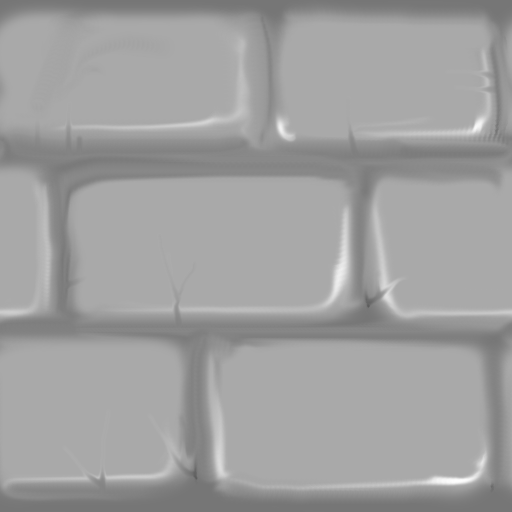
\includegraphics[width=0.2\textwidth]{Wall}
    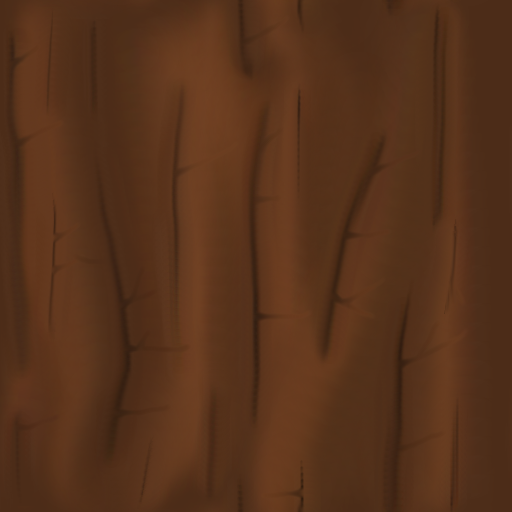
\includegraphics[width=0.2\textwidth]{Wood}
    \caption{Textures}
\end{figure}

Les textures liées aux modèles 3D ont été “faites mains” grâce aux outils que proposaient blender et Krita, un logiciel opensource de peinture numérique. Un bonus serait de pouvoir rajouter une “normal Map” pour donner des effets de relief et proposer ainsi un meilleur rendu.

\begin{figure}[H]
    \centering
    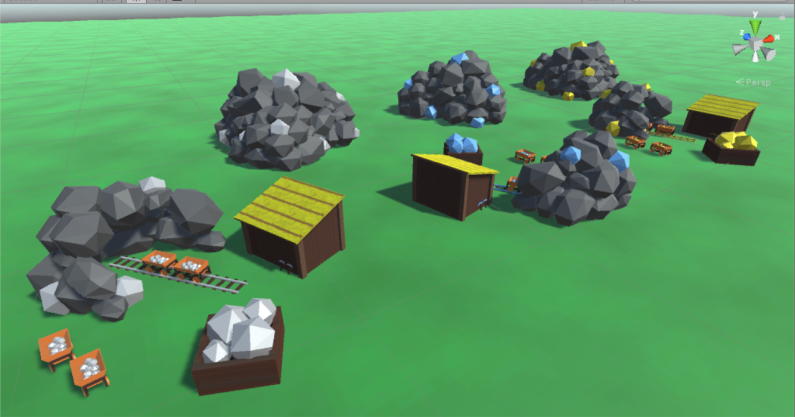
\includegraphics[scale=0.8]{mines}
    \caption{Exemple de feature: les mines}
\end{figure}

\section{Interface (Thibault \& Valérian)}

En ce qui concerne l’interface actuelle, il ne s’agit que d’une version créée rapidement afin de tester rapidement les fonctionnalitées qui sont implémentées, faisant fi de l’esthétique. Cette interface test permet de se rendre compte des besoins qui seront à prendre en compte dans la version finale afin d’augmenter l'ergonomie des menus. Dans la version finale, il ne restera presque rien de l'interface actuelle, qui permet juste aux différents membres de tester leur propre partie.

Actuellement, le menu d’accueil est constitué uniquement des boutons, d’un slider pour sélectionner le nombre de joueurs et de champs d’entrée textuelles servant à récupérer l’IP pour une connexion au serveur et le nom du joueur.

Du côté de l’interface en jeu, il s’agit de boutons permettant de sélectionner des options de modifications de la carte de jeu, ainsi qu’un menu permettant d'accéder à la sauvegarde.

Il est à noter que nous avons opté pour une interface français/anglais afin de toucher une population plus vaste en laissant l'option d'un langage largement répandu.

\section{Site Web (Valérian)}

En l’état actuel, le site possède un design basique permettant d’avoir une idée de son futur, ainsi qu’une page d’accueil fournissant des liens à tous les éléments nécessaires, que ce soit des logiciels utilisés, au jeu en lui même, en passant par les rapports de soutenance. Il est hébergé grâce au service GitHub Pages.\\
La page d’accueil du site, se présente sous la forme suivante :

\begin{figure}[H]
    \centering
    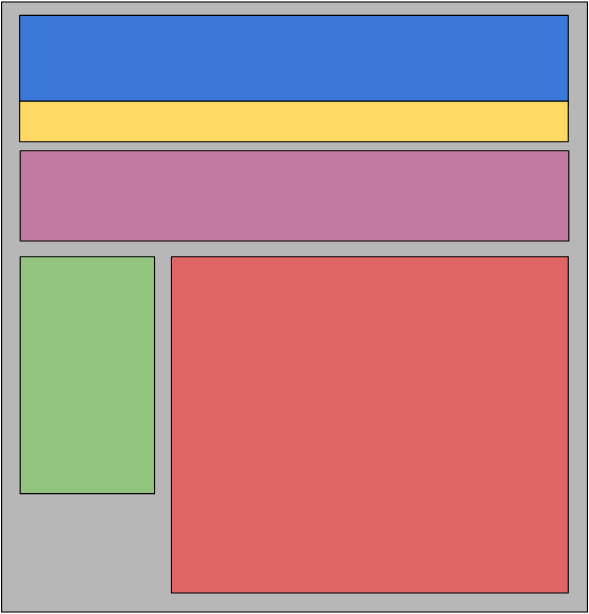
\includegraphics[scale=0.8]{layout_website}
    \caption{Mise en page du site web}
\end{figure}

La zone bleu étant le titre du jeu, la jaune le menu permettant de joindre les différentes autres pages, la violette un bandeau image,la verte une liste de liens utiles comme les logiciels ou les téléchargements et la zone rouge sera remplie au fur et à mesure avec des notes de mise à jour, permettant de suivre l’avancé du projet.

Les autres pages du site suivent la même structure, en modifiant toutefois le contenu de la zone rouge en fonction du but de la page, et en modifiant ou supprimant la zone verte selon nécessité.

Un plan du site à été envisagé comme suit :

\begin{itemize}
	\item Page d'accueil
	\begin{itemize}
	\item Présentation du jeu
	\item Comment jouer ?
		\begin{itemize}
		\item Solo
		\item Multijoueur
		\end{itemize}
	\item Ressources utilisées
		\begin{itemize}
		\item Textures
		\item Sons
		\item Logiciels
		\item Autres assets
		\end{itemize}
	\item Présentation de l'équipe
		\begin{itemize}
		\item Thibault Allançon
		\item Valérian Fayt
		\item Cédric Parpet
		\item Antoine Gonzalez
		\end{itemize}
	\item Notes de mises à jour
	\item Téléchargements
		\begin{itemize}
		\item Cahier des charges
		\item Rapports de soutenance
		\item Jeu
		\end{itemize}
	\end{itemize}
\end{itemize}


\chapter{Avances, retards, difficultées rencontrées}

\section*{Map}

Pas de retard ou d'avance.

\section*{Multijoueur}

La progression du multijoueur suit les objectifs qui lui étaient fixés, c’est à dire d’établir une connection entre les joueurs et de pouvoir transmettre des informations entre eux. Atteindre cet objectif n’a pas été simple car il a été nécessaire de se plonger dans un univers encore inconnu dans lequel nous n’avions aucune notion. Il a premièrement été envisagé d’utiliser la base de multiplayer que propose Unity toutefois nous nous sommes vite retrouvé coincé par des difficultées techniques concernant la synchronisation de la map dans le jeu. Réalisant que ces difficultés risquaient de poser problème plus tard dans le développement du jeu, nous avons opté pour une toute autre voie, construire notre propre système de serveur/clients. Appuyé par l’idée d’apprendre quelque chose de nouveau, il a fallu parcourir de nombreuses documentations et suivre plusieurs tutoriels sur le sujet pour parvenir à une base solide et fonctionnelle. La seconde difficulté, plus mineure, a été de tenter de prévoir les différents cas possibles lors des connections, afin de prévenir du maximum d’erreurs. La résolution de cette difficulté à été simplifié en tentant un maximum de cas possible et modifiant l’implémentation en conséquence.

\section*{Gameplay}

Tout ce qui était prévu a été fait. J'aurais préféré commencer à implémenter des éléments afin d'obtenir quelque chose de concret dans le jeu, mais les shémas, tableaux et diagrames me permettront de gagner beaucoup de temps lors de l'implémentation à venir. Le code ne sera pas bien compliqué, maintenant que tous les éléments sont prévus.

\section*{Autre}

\begin{itemize}
    \item \textbf{Assets :} La modélisation étant compliqué à faire et chronophage, le nombre d’asset créé n’est pas suffisant pour atteindre les 50\% voulu lors de la première soutenance. On se situerais plutôt entre 35 et 40\%. Le processus de fabrication des assets devrait cependant être beaucoup plus rapide pour la suite.
    \item \textbf{Interface :} N’ayant pas établis d’objectif visuels pour l’interface à ce niveau de développement, nous ne voulions qu’avoir des menus permettant de tester les fonctionnalitées que nous implémentions. Cet objectif a été rempli.
    \item \textbf{Site web :} En avance.
\end{itemize}

\chapter{A venir}

\begin{itemize}
	\item \textbf{Map :} Intégrer les unités, système de génération aléatoire de map
	\item \textbf{Multijoueur :} Transmettre la map originale, éventuellement accumuler les messages pour diminuer la quantité de données à envoyer.
	\item \textbf{Gameplay :} Implémentation des classes, gestion des messages pour le multijoueur, commencer à équilibrer l’économie.
	\item \textbf{Assets :} Créations des autres assets pour compléter le jeu. Ajout des armatures sur les unités pour les animations de déplacement et de combat. Ajout de petits effets visuels (scintillement pour les mines, feu de camp) pour étoffer les modèles et utiliser le système de particules offert par unity.
	\item \textbf{Interface :} Menu principal clair, début de menu in-game, implémentation du changement de langue.
	\item \textbf{Site Web :} Compléter le site avec les pages manquantes
\end{itemize}

\chapter{Expériences personnelles}

\begin{itemize}
	\item \textbf{Thibault :} L’implémentation de la map m’a permis d’apprendre concrètement à utiliser Unity, et le fait de voir évoluer son propre jeu ainsi que les fonctionnalités qu’on développe rend cet apprentissage d’autant plus agréable et motivant pour la suite. Le fait que la map soit constituée d’hexagones a constitué un certain challenge pour le rendu visuel, la triangulation et le pavage.
	\item \textbf{Valérian :} Travailler sur ce projet pendant les mois qui ont précédés à été une expérience fortement intéressante et instructive. J’ai pu en effet découvrir comment manipuler certains outils tels que GitHub et Unity, mais ai aussi appris beaucoup concernant la programmation en général. Les parties dont j’ai pu m’occuper, notamment le réseau, m’ont permis d’apprendre des choses qui m'étaient totalement inconnues, et incité à chercher de la documentation plus poussée. J’ai aussi pu faire face à des problèmes qui m’ont beaucoup appris et grâce auquel je retire une expérience nouvelle. J’ai trouvé particulièrement plaisant le fait de voir le projet se construire peu à peu, chaque semaine un peu plus complet. Satisfait de mon organisation dans le temps et du travail que j’ai fournis, je compte renouveler cette bonne expérience pour les mois qui suivent.
	\item \textbf{Cédric :} Cette première période fut assez difficile pour ma part. Je m’étais pris à la création des asset 3D assez tard ce qui est une des raisons de mon retard sur ce qui était prévu. Néanmoins je suis très heureux d’avoir pu utiliser les compétences que je possédais déjà sur blender car la modélisation et l’animation 3D sont des domaines que j’apprécie énormément. J’ai également appris de nouvelles techniques et suis devenu plus rapide sur mes créations. Je suis assez satisfait de ce que j’ai fait et je compte bien faire mieux plus tard. Le retard que j’ai pris m’aura au moins appris qu’il est essentiel de travailler sur le projet chaque semaine. D’autant plus que je dois également m’occuper de l’interface du jeu qui sera plus complexe que celle qui est actuellement disponible.
	\item \textbf{Antoine :} Période vraiment intéressante, qui m’a permis de réaliser à quel point faire un jeu (ou une application en général) relève d’abord d’une phase de réflexion importante pendant laquelle il faut planifier toutes les éventualités et les buts du projet. On voit le jeu prendre une direction, et on sait à quoi s’attendre dans les semaines qui viennent sans s’inquiéter de devoir ajouter/supprimer/modifier des bouts de code toutes les 5 minutes.
\end{itemize}

\chapter{Conclusion}

Cette première partie du projet s'achève donc sur un ressenti positif de notre part. Le projet avance à un rythme correct, les éléments implémentés fonctionnent, les éléments pas encore implémentés sont déjà prévus et pensés, et la difficulté du démarage ne nous aura pas handicapé autant que nous l'aurions imaginés. C'est donc plein de volonté et de positivité que nous pouvons commencer la deuxième phase.

\end{document}
